\fixme{\bf The figure in this subsection will be improved for the next version of the draft.}

The front-end (FE) ASIC, also known as LArASIC, receives signals from the CR board and
provides a means to amplify and shape the signals originally coming from the TPC wires; the
shaping serves as an anti-aliasing filter for the TPC signals.
Each LArASIC channel has a charge amplifier circuit with a programmable
gain selectable from one of 4.7, 7.8, 14 and 25~mV/fC
(full scale charge of 55, 100, 180 and 300~fC),
a high-order anti-aliasing filter with programmable time
constant (semi-Gaussian with peaking time 0.5, 1, 2, and 3 $\mathrm{\mu}$s),
an option to enable AC coupling,
and a baseline adjustment for operation with either the collecting (200~mV) or the non-collecting (900~mV) wires.
Shared among the 16 channels in the FE ASIC are the bias circuits, programming registers,
a temperature monitor, an analog buffer for signal monitoring, and the digital interface.
The power dissipation of LArASIC is about 6~mW per channel at 1.8~V supply.

LArASIC is implemented using the TSMC 180 nm CMOS process.  The charge sensitive amplifier uses a very large PFET (width = 20 mm, length = 270 nm) followed by a dual cascode stage, a pulse shaping network, and a baseline restoration circuit.  

Each channel also implements a high-performance output driver,
which can be used to drive a long cable, but is disabled when interfaced to an ADC ASIC to reduce the power consumption.
The ASIC integrates a band-gap reference (BGR) to generate all the internal bias voltages and currents.
This guarantees a high stability of the operating point over a wide range of
temperatures, including cryogenic.
The ASIC is packaged in a commercial, fully encapsulated plastic QFP 80 package.

Each FE ASIC channel is equipped with an injection capacitor which can be used
for test and calibration and can be enabled or disabled through a
dedicated register. The injection capacitance has been measured using 
a calibrated external capacitor. The measurements show
that the calibration capacitance is extremely stable, changing from
184~fF at RT to 183~fF at 77~K. This result and the measured
stability of the peaking time demonstrate the high stability of the
passive components as a function of temperature. Channel-to-channel and chip-to-chip
variation in the calibration capacitor are typically less than 1\%. 

\begin{dunefigure}
[Measured pulse response with details on gain, peaking time and baseline adjustments.]
{fig:fe-output}
{Measured pulse response with details on gain, peaking time and baseline adjustments.}
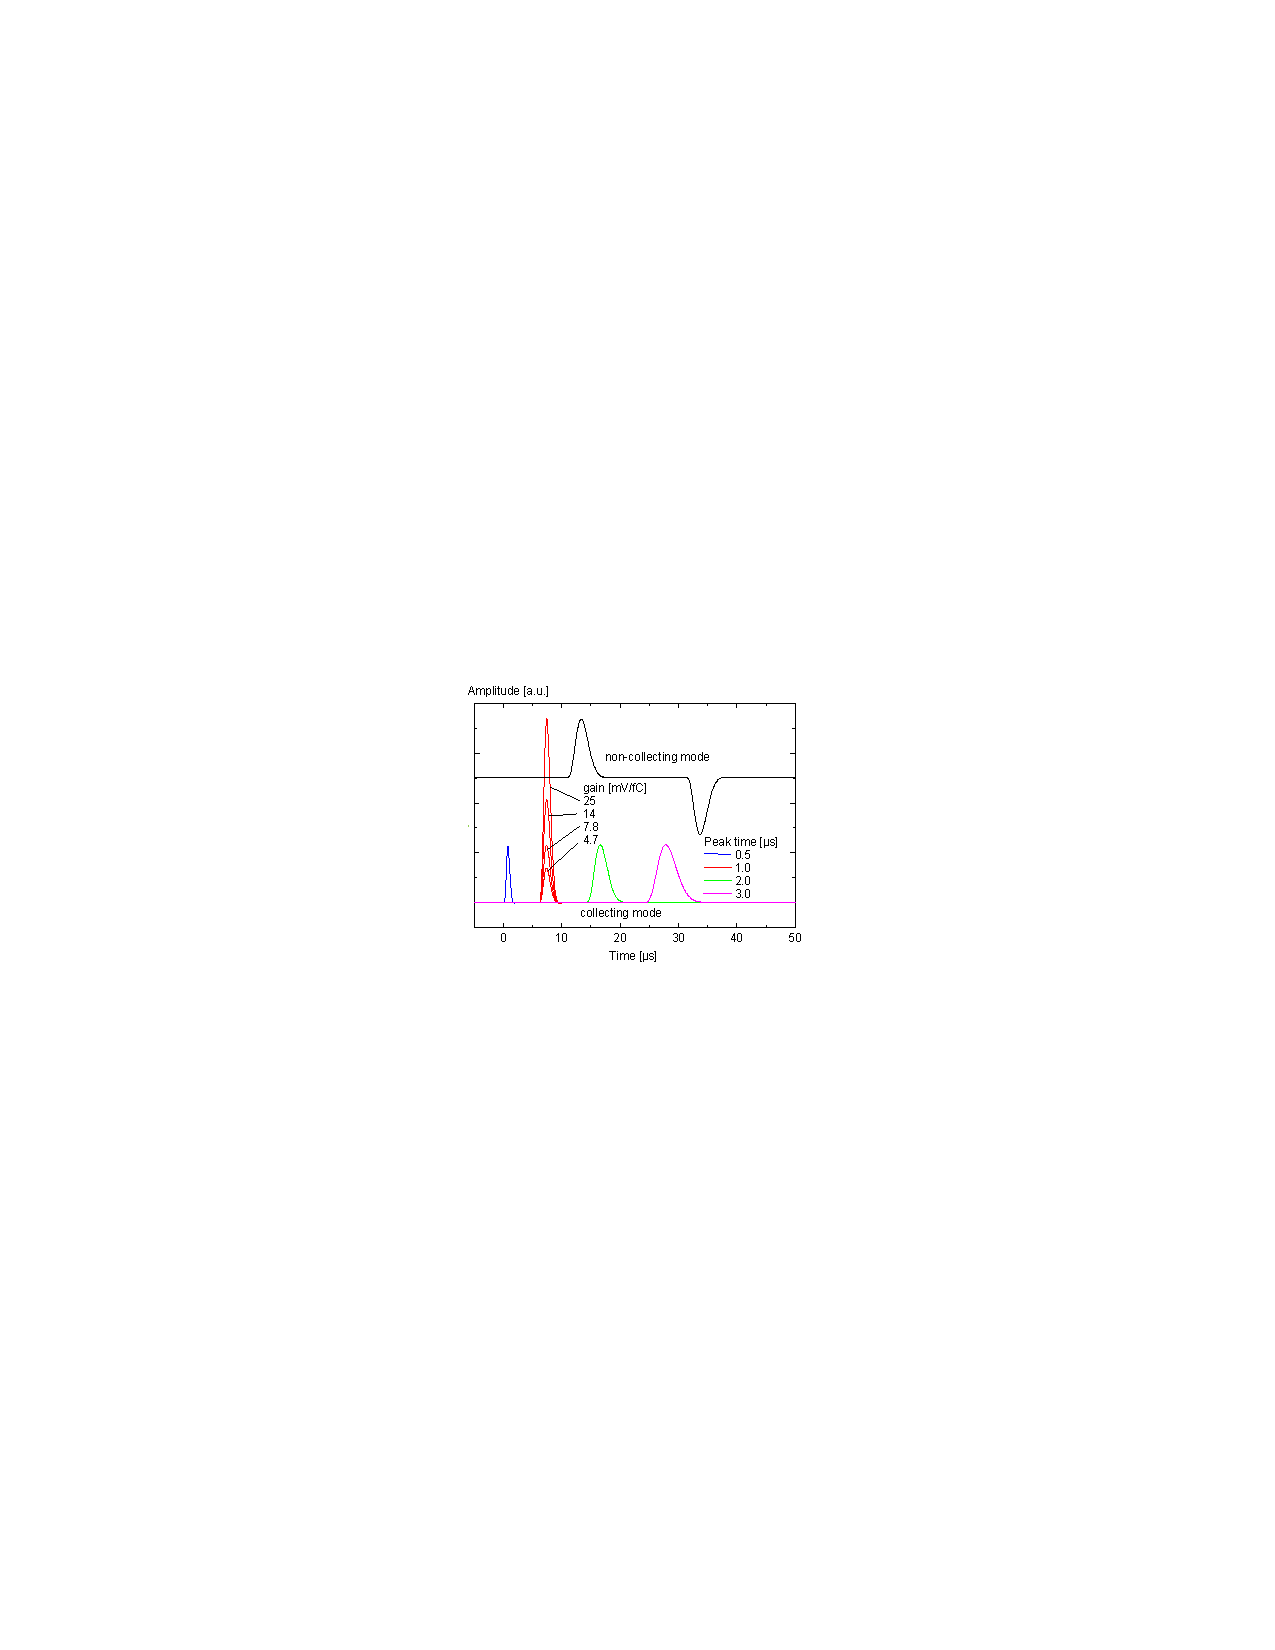
\includegraphics[width=0.85\linewidth]{tpcelec-shaper_out.pdf}
\end{dunefigure}

Prototype ASICs have been evaluated and characterized at RT (300~K) and LN2 (77~K) temperature.
During testing the circuits have been cycled multiple times
between the two temperatures and operated without any change in performance.
Figure~\ref{fig:fe-output} shows the measured pulse response, both as a function
of temperature and the programmable settings of the chip.
These results are in close agreement with simulations and indicate
that both the analog and the digital circuits and interface operate as
expected in a cryogenic environment.
